\documentclass[twocolumn, 12pt]{article}

\usepackage[utf8]{inputenc}
\usepackage[english, spanish]{babel}
\usepackage[papersize={216mm,330mm},tmargin=15mm,bmargin=15mm,lmargin=15mm,rmargin=15mm]{geometry}
\usepackage{fullpage}
\usepackage{graphicx}
\usepackage{amsmath}
\usepackage{enumitem}
\usepackage{chngcntr}
\usepackage{setspace}
\usepackage{url}
\usepackage{csquotes}
\usepackage{float}
\usepackage{verbatim}
\usepackage{tabularx}
\usepackage{amsmath}
\usepackage{caption}

\counterwithin{figure}{section}
\renewcommand{\thesection}{\arabic{section}}
\renewcommand{\thesubsection}{\thesection.\arabic{subsection}}
\renewcommand{\baselinestretch}{1.5}

\usepackage[style=apa, maxnames=6, minnames=3, backend=biber]{biblatex}
\DefineBibliographyStrings{english}{%chktex-file 1 chktex-file 6
    andothers = {\em et\addabbrvspace al\adddot}
}
\addbibresource{./Bibliography/bibliography.bib}

\usepackage{array}
\usepackage{enumitem}
\usepackage{longtable}

\setlength{\parskip}{0pt}

\raggedbottom{}

\begin{document}

\begin{titlepage}
    \centering
    
\includegraphics[width=0.3\textwidth]{Images/logo_utb.png}\par\vspace{1cm}
    {\scshape\LARGE Universidad Tecnológica de Bolívar \par}
    \vspace{1.5cm}

    {\scshape\Large FÍSICA ELÉCTRICA \par}
    \vspace{.2cm}

    % chktex-file 8
    \vspace{2cm}
    % chktex-file 8
    \slshape {\Large \bfseries{} RC CIRCUIT SIMULATION\\}
    \vspace{3cm}

    \slshape {\itshape{} Mauro González, T67622 \\}
    \slshape {\itshape{} German De Armas Castaño, T68765 \\}
    \slshape {\itshape{} Angel Vega Rodriguez, T68186 \\}
    \slshape {\itshape{} Juan Jose Osorio Ariza, T67316 \\}
    \vfill

    Revisado Por \\ David Sierra Porta \\

    {\large \today\par}
\end{titlepage}

~\nocite{GoogleDrive}

% -----------------------------------------------------------|>
\section{Datos experimentales}

\begin{table}[H]
    \captionsetup{justification=centering}
    \centering

    % chktex-file 44
    \begin{tabularx}{0.9\linewidth}{|>{\centering\arraybackslash}X|>{\centering\arraybackslash}X|}
        \hline
        \multicolumn{2}{|c|}{Constantes}              \\ \hline

        $\varepsilon$ \textit{(V)}            & $30$  \\\hline
        Resistencia \textit{($\Omega$)}       & $80$  \\\hline
        Capacitancia \textit{($\mathcal{F}$)} & $0.2$ \\\hline
        RC \textit{($\tau$)} \textit{[Seg]}   & $16$  \\\hline
    \end{tabularx}

\end{table}

\begin{table}[H]
    \centering
    \begin{tabularx}{0.9\linewidth}{|>{\centering\arraybackslash}X|>{\centering\arraybackslash}X|}

        \hline
        \multicolumn{2}{|c|}{Carga}                  \\\hline
        Tiempo \textbf{[Seg]} & Voltaje \textbf{[V]} \\\hline
        $0.0$                 & $0.0$                \\\hline
        $5.5$                 & $9.65$               \\\hline
        $10.4$                & $15.01$              \\\hline
        $15.6$                & $19.15$              \\\hline
        $20.2$                & $21.9$               \\\hline
        $25.4$                & $24.13$              \\\hline
        $30.4$                & $25.73$              \\\hline
        $35.5$                & $26.89$              \\\hline
        $40.3$                & $27.7$               \\\hline
        $45.3$                & $28.31$              \\\hline
        $50.4$                & $28.77$              \\\hline
        $55.5$                & $29.11$              \\\hline
        $60.3$                & $29.34$              \\\hline
        $65.5$                & $29.52$              \\\hline
        $70.3$                & $29.65$              \\\hline
        $75.5$                & $29.75$              \\\hline
        $80.3$                & $29.81$              \\\hline
        $85.6$                & $29.86$              \\\hline
        $90.5$                & $29.9$               \\\hline
        $95.5$                & $29.93$              \\\hline
        $100.4$               & $29.95$              \\\hline
    \end{tabularx}

    % chktex-file 24
    \caption{Carga del capacitor}
    \label{tab:datos__Carga}
\end{table}

\begin{figure}[H]
    \centering
    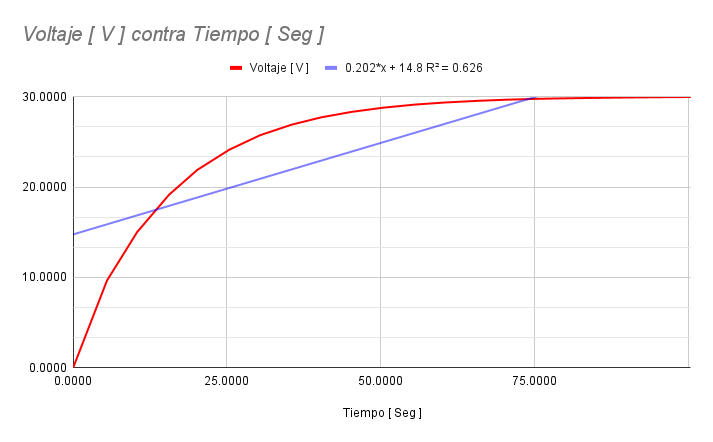
\includegraphics[width=\linewidth]{./Images/Voltaje [ V ] contra Tiempo [ Seg ].png}
\end{figure}

\begin{itemize}[label=$\triangleright$]
    \item Linea de tendencia:\hfill \break{} $y = 0.202x + 14.8$
\end{itemize}

\begin{table}[H]
    \centering
    \begin{tabularx}{0.9\linewidth}{|>{\centering\arraybackslash}X|>{\centering\arraybackslash}X|}

        \hline
        Tiempo \textbf{[Seg]} & $\ln (1- \frac{V}{\varepsilon})$ \\\hline
        $0.00$                & $0$                              \\\hline
        $5.50$                & $-0.38812$                       \\\hline
        $10.40$               & $-0.69381$                       \\\hline
        $15.60$               & $-1.01703$                       \\\hline
        $20.20$               & $-1.30933$                       \\\hline
        $25.40$               & $-1.63134$                       \\\hline
        $30.40$               & $-1.94958$                       \\\hline
        $35.50$               & $-2.26657$                       \\\hline
        $40.30$               & $-2.56829$                       \\\hline
        $45.30$               & $-2.87647$                       \\\hline
        $50.40$               & $-3.19418$                       \\\hline
        $55.50$               & $-3.51773$                       \\\hline
        $60.30$               & $-3.81671$                       \\\hline
        $65.50$               & $-4.13517$                       \\\hline
        $70.30$               & $-4.45102$                       \\\hline
        $75.50$               & $-4.78749$                       \\\hline
        $80.30$               & $-5.06193$                       \\\hline
        $85.60$               & $-5.36731$                       \\\hline
        $90.50$               & $-5.70378$                       \\\hline
        $95.50$               & $-6.06046$                       \\\hline
        $100.40$              & $-6.39693$                       \\\hline

    \end{tabularx}

    % chktex-file 24
    \caption{$y = mx$}
    \label{tab:yEqualsMX__Carga}
\end{table}

\begin{figure}[H]
    \centering
    % chktex-file 36
    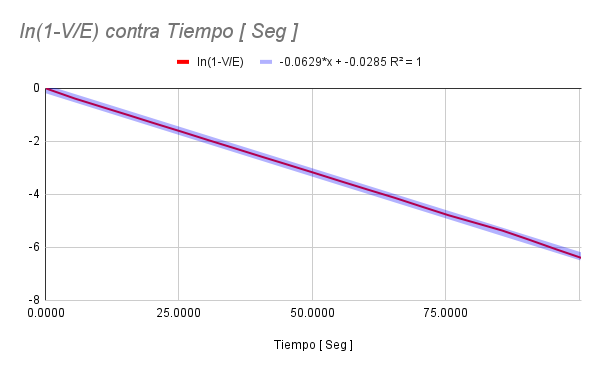
\includegraphics[width=\linewidth]{./Images/ln(1-V_E) contra Tiempo [ Seg ].png}
\end{figure}

\begin{itemize}[label=$\triangleright$]
    \item Linea de tendencia:\hfill \break{} $y = -0.0629x -0.0285$
\end{itemize}

\begin{table}[H]
    \centering
    \begin{tabularx}{0.9\linewidth}{|>{\centering\arraybackslash}X|>{\centering\arraybackslash}X|}

        \hline
        \multicolumn{2}{|c|}{Descarga}               \\\hline
        Tiempo \textbf{[Seg]} & Voltaje \textbf{[V]} \\\hline
        $0.0$                 & $29.99$              \\\hline
        $5.5$                 & $20.82$              \\\hline
        $10.3$                & $15.26$              \\\hline
        $15.5$                & $11.0$               \\\hline
        $20.3$                & $8.17$               \\\hline
        $25.3$                & $5.97$               \\\hline
        $30.3$                & $4.35$               \\\hline
        $35.5$                & $3.14$               \\\hline
        $40.3$                & $2.33$               \\\hline
        $45.4$                & $1.0$                \\\hline
        $50.3$                & $1.24$               \\\hline
        $55.3$                & $0.91$               \\\hline
        $60.3$                & $0.67$               \\\hline
        $65.4$                & $0.49$               \\\hline
        $70.3$                & $0.36$               \\\hline
        $75.2$                & $0.26$               \\\hline
        $80.3$                & $0.19$               \\\hline
        $85.3$                & $0.14$               \\\hline
        $90.6$                & $0.1$                \\\hline
        $95.3$                & $0.07$               \\\hline
        $100.2$               & $0.05$               \\\hline
    \end{tabularx}

    % chktex-file 24
    \caption{Descarga del capacitor}
    \label{tab:datos__Descarga}
\end{table}

\begin{figure}[H]
    \centering
    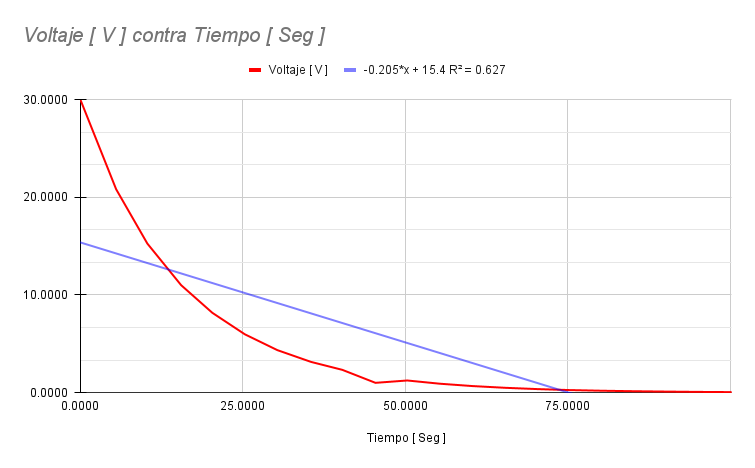
\includegraphics[width=\linewidth]{./Images/Voltaje [ V ] contra Tiempo [ Seg ] Descarga.png}
\end{figure}

\begin{itemize}[label=$\triangleright$]
    \item Linea de tendencia:\hfill \break{} $y= -0.205x + 15.4$
\end{itemize}

\begin{table}[H]
    \centering
    \begin{tabularx}{0.9\linewidth}{|>{\centering\arraybackslash}X|>{\centering\arraybackslash}X|}

        \hline
        Tiempo \textbf{[Seg]} & $\ln(\frac{V}{\varepsilon})$ \\\hline
        $0.00$                & $-0.0003$                    \\\hline
        $5.50$                & $-0.3653$                    \\\hline
        $10.30$               & $-0.6760$                    \\\hline
        $15.50$               & $-1.0033$                    \\\hline
        $20.30$               & $-1.3007$                    \\\hline
        $25.30$               & $-1.6145$                    \\\hline
        $30.30$               & $-1.9310$                    \\\hline
        $35.50$               & $-2.2570$                    \\\hline
        $40.30$               & $-2.5553$                    \\\hline
        $45.40$               & $-3.4012$                    \\\hline
        $50.30$               & $-3.1861$                    \\\hline
        $55.30$               & $-3.4955$                    \\\hline
        $60.30$               & $-3.8017$                    \\\hline
        $65.40$               & $-4.1145$                    \\\hline
        $70.30$               & $-4.4228$                    \\\hline
        $75.20$               & $-4.7483$                    \\\hline
        $80.30$               & $-5.0619$                    \\\hline
        $85.30$               & $-5.3673$                    \\\hline
        $90.60$               & $-5.7038$                    \\\hline
        $95.30$               & $-6.0605$                    \\\hline
        $100.20$              & $-6.3969$                    \\\hline
    \end{tabularx}

    % chktex-file 24
    \caption{$y = mx$}
    \label{tab:yEqualsMX__Descarga}
\end{table}

\begin{figure}[H]
    \centering
    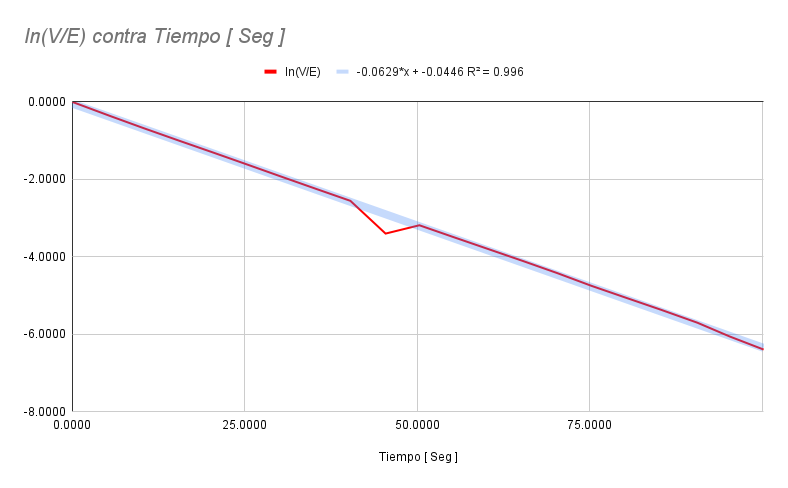
\includegraphics[width=\linewidth]{./Images/ln(V_E) contra Tiempo [ Seg ] Descarga.png}
\end{figure}

\begin{itemize}[label=$\triangleright$]
    \item Linea de tendencia:\hfill \break{} $y= -0.0629x -0.0446$
\end{itemize}

% -----------------------------------------------------------|>
\section{Charging a capacitor}

% ----------------------------------------|>
\subsection{Using the equations above what is the time constant $\tau$? (Seg)}

Usando la ecuación,

{\large
        \begin{equation}
            \tau = R \cdot C
            \label{eq:Tau}
        \end{equation}
    }

tenemos, $\tau = 80 \Omega \cdot 0.2 \mathcal{F} = 16 Seg$

% ----------------------------------------|>
\subsection{When t = $\tau$ what is the value of the voltage? (V)}

Usando la ecuación,

{\large
        \begin{equation}
            V_c = \frac{q}{c} = \varepsilon (1 - e^{\frac{-t}{RC}})
            \label{eq:voltaje__Carga}
        \end{equation}
    }

$V_c = 30V (1 - e^{-1}) = 18.9636V$

% ----------------------------------------|>
\subsection{What percentage of the battery voltage is the voltage across the capacitor at this time?}

Usando la ecuación~\eqref{eq:voltaje__Carga} despejada,

{\large
        \begin{equation}
            \frac{V_c}{\varepsilon} = 1 - e^{\frac{-t}{RC}}
            \label{eq:voltaje__Carga-Porcentaje}
        \end{equation}
    }

Si $t = \tau$, $\frac{V_c}{\varepsilon} = 1 - e^{-1} =
    63.21\%$

% ----------------------------------------|>
\subsection{When t = $2\tau$ what is the value of the voltage? (V)}

Según la ecuación~\eqref{eq:voltaje__Carga}, $V_c = 30V (1
    - e^{-2}) = 25.9399V$

% ----------------------------------------|>
\subsection{What percentage of the battery voltage is the voltage across the capacitor at this time?}

Si $t = 2\tau$, $\frac{V_c}{\varepsilon} = 1 - e^{-2} =
    86.46\%$

% ----------------------------------------|>
\subsection{By what percentage of the battery voltage did the voltage across the capacitor change from
    t = $\tau$ to t = $2\tau$?}

{\large
    \begin{equation}
        \% = \frac{NuevoValor - ValorInicial}{ValorInicial} \cdot 100
        \label{eq:porcentajeCambio}
    \end{equation}
}

Desde t = $t$ a t = $2\tau$, $\% = \frac{25.9399V -
        18.9636V}{18.9636V} \cdot 100 = 36.7878\%$

% ----------------------------------------|>
\subsection{Is the following statement true: During charging, the capacitor gains the largest fraction of
    its final voltage during the time t = $\tau$ to t = $2\tau$?}

La afirmación es incorrecta debido a que, en el intervalo
de tiempo desde t = $0$ hasta t = $2\tau$, el capacitor
gana un $\sim 63\%$ de su carga total, mientras que en el
intervalo desde t = $\tau$ hasta t = $2\tau$, pasa de un
$\sim 63\%$ a un $\sim 86\%$.

Siguiendo esta tendencia, aunque t = $3\tau$, t=$4\tau$,
t=$n\tau$ \dots{},el capacitor va a ir ganando cada vez
menos voltaje, siendo asi, el intervalo hasta t=$\tau$ el
momento en el que gana mas porcentaje de la carga total.

% ----------------------------------------|>
\subsection{Looking at the plot, at about what time did the voltage reach 63\% of its total voltage? (Seg)}

Según la tabla~\ref{tab:datos__Carga}, alrededor de los
$15.6$ Seg, el capacitor ganó un $63\%$ de la carga total,
siendo $19.15V$

% ----------------------------------------|>
\subsection{Assume you do not know the value of the capacitor C, calculate C from the knowledge of
    R and time constant found in question 1. (F)}

Despejando $C$ de la ecuación~\eqref{eq:Tau}, $C =
    \frac{\tau}{R} = \frac{16 Seg}{80} = 0.2 \mathcal{F}$

% ----------------------------------------|>
\subsection{What is the percent error between the calculated value and the exact value of C?}

En este contexto, el porcentaje de error es de 0\%, debido
a que los valores calculados y teóricos para $C$ son
exactamente los mismos. Dicho de otra forma,

$\% = \frac{0.2 - 0.2}{0.2} \cdot 100 = 0\%$

% ----------------------------------------|>
\subsection{Write your result as y =m x, what is the value of m? (1/s)}

Basado en los datos de la tabla~\ref{tab:datos__Carga}, $y
    = 0.202x + 14.8$

% ----------------------------------------|>
\subsection{Using your plot and the result from question 4, what value of $\tau$ do you find? (s)}

Según los datos de la tabla~\ref{tab:datos__Carga}, el
voltaje de $25.9V$ se encuentra alrededor de los $\sim
    32.5$ Seg. Considerando que $t = 16$ Seg, $\frac{32.5}{16}
    = 2.03 \tau$

% ----------------------------------------|>
\subsection{Again assuming we do not know the capacitance solve for C using your fitted value of $\tau$
    and the known value of R. (F)}

Despejando $C$, de la ecuación~\eqref{eq:Tau},

$C = \frac{\tau}{R} = \frac{32.5}{80} = 0.406 \mathcal{F}$

% ----------------------------------------|>
\subsection{What is the percent error between the calculated value and the exact value of C?}

$\% = \frac{0.406 - 0.2}{0.2} \cdot 100 = 103\%$

% -----------------------------------------------------------|>
\section{Discharging a Capacitor}

% ----------------------------------------|>
\subsection{Is the time constant $\tau$ different when we discharge a capacitor?}

No, la constante de tiempo ($\tau$) es la misma tanto
cuando cargamos como cuando descargamos un condensador. La
constante de tiempo es una propiedad característica del
circuito RC y está determinada por los valores de la
resistencia (R) y la capacitancia (C) en el circuito.
Representa el tiempo que tarda la tensión a través del
condensador en alcanzar aproximadamente el 63,2\% de su
valor final durante la carga y disminuir a aproximadamente
el 36,8\% de su valor inicial durante la descarga.

% ----------------------------------------|>
\subsection{When t = $\tau$ what is the value of the voltage?}

Usando la ecuación,

{\large
        \begin{equation}
            V_c = \varepsilon \cdot e^{\frac{-t}{RC}}
        \end{equation}
        \label{eq:descarga}
    }

$V_c = 30 \cdot e^{-1} = 11.036V$

% ----------------------------------------|>
\subsection{What percentage of the battery voltage is the voltage across the capacitor at this time?}

Usando la ecuación~\eqref{eq:descarga} despejada,

{\large
        \begin{equation}
            \frac{V_c}{\varepsilon} = e^{\frac{-t}{RC}}
        \end{equation}
        \label{eq:descarga__porcentaje}
    }

Si t = $\tau$, $\frac{V_c}{\varepsilon} = e^{-1} = 36.78\%$

% ----------------------------------------|>
\subsection{When t = $2\tau$ what is the value of the voltage? (V)}

Según la ecuación~\eqref{eq:descarga}, $V_c = 30 \cdot
    e^{-2} = 4.060V$

% ----------------------------------------|>
\subsection{What percentage of the battery voltage is the voltage across the capacitor at this time?}

Según la ecuación~\eqref{eq:descarga__porcentaje},
$\frac{V_c}{\varepsilon} = e^{-2} = 13.53\%$

% ----------------------------------------|>
\subsection{By what percentage of the battery voltage did the voltage across the capacitor change
    from t = $\tau$ to t = $2\tau$?}

Usando la ecuación~\eqref{eq:porcentajeCambio}, $\% =
    \frac{4.060 - 11.036}{11.036} \cdot 100 = -63.211\%$
\footnote{El negativo indica que la corriente esta
    disminuyendo}

% ----------------------------------------|>
\subsection{Is the following statement true: During discharging the capacitor loses the largest
    fraction of its initial voltage during the time t = $\tau$ to t = $2\tau$}

Durante la descarga de un capacitor, es incorrecto afirmar
que el capacitor pierde la mayor fracción de su voltaje
inicial durante el tiempo t = $\tau$ hasta t = $2\tau$. En
realidad, la mayor fracción de pérdida de voltaje ocurre
durante el intervalo de tiempo desde t = $0$ hasta t =
$\tau$.

De acuerdo con la constante de tiempo RC, que determina el
comportamiento de carga y descarga del capacitor, durante
la descarga el capacitor experimenta una disminución
exponencial en su voltaje. Durante el intervalo desde t = 0
hasta t = $\tau$, aproximadamente el 63,2\% de la carga
inicial del capacitor se ha perdido. Esto se debe a que la
descarga sigue una curva exponencialmente decreciente.

Sin embargo, a medida que avanzamos desde t = $\tau$ hasta
t = $2\tau$, el capacitor continúa perdiendo carga, pero la
fracción de pérdida de voltaje en este intervalo es menor
en comparación con el intervalo anterior. Por lo tanto, el
intervalo desde t = 0 hasta t = $\tau$ es cuando el
capacitor experimenta la mayor fracción de pérdida de su
voltaje inicial durante la descarga.

% ----------------------------------------|>
\subsection{Looking at the plot at about what time did the voltage reach 36.8\% of its total voltage?
    (s)}

Según la tabla~\ref{tab:datos__Descarga}, alrededor de los
$15$ Seg, el capacitor perdió un $63\%$ del voltaje total.

% ----------------------------------------|>
\subsection{Assume you do not know the value of the resistor R, calculate R from the knowledge of
    C and the time constant found in question 1}

Despejando $R$ de la ecuación~\eqref{eq:Tau},

{\large
        \begin{equation}
            R = \frac{\tau}{C}
        \end{equation}
    }

$R = \frac{16 Seg}{0.2\mathcal{F}} = 80 \Omega$

% ----------------------------------------|>
\subsection{What is the percent error between the calculated values and the exact value of R?}

En este contexto, el valor teórico y calculado para $R$ son
exactamente los mismos, es decir, un 0\% de diferencia
entre los valores.

% ----------------------------------------|>
\subsection{Write your result as y = mx, what is the value of m? (1/s)}

Basado en los datos de la tabla~\ref{tab:datos__Descarga},
$y= -0.205x + 15.4$

% ----------------------------------------|>
\subsection{Using your plot and the result from question 11, what value of $\tau$ do you find? (s)}

Usando la ecuación de la linea de tendencia
de~\ref{tab:datos__Carga}, evaluado en $\tau$, da un valor
de $13.75$ Seg.

% ----------------------------------------|>
\subsection{Again assuming we do not know resistance solve for R using your fitted value of $\tau$ and
    the known value of C. ($\Omega$)}

Despejando $R$ de~\eqref{eq:Tau}, $R = \frac{\tau}{C} =
    \frac{13.75}{0.2} = 68.75 \Omega$

% ----------------------------------------|>
\subsection{What is the percent error between the calculated value and the exact value of R?}

$\% = \frac{80 - 68.75}{68.75} \cdot 100 = 16.36\%$

% -----------------------------------------------------------|>
\section{Non-Ohmic Materials}

% ----------------------------------------|>
\subsection{As you turn on a light switch, does the resistance of a light bulb stay constant?}

De acuerdo con los resultados obtenidos mediante el
simulador utilizado, se observa que la resistencia del
bombillo se mantiene constante sin importar la variación
del voltaje. Cabe mencionar que en aplicaciones prácticas,
como en el caso de las bombillas incandescentes, la
resistencia puede experimentar cambios debido al efecto de
calentamiento del filamento.

% ----------------------------------------|>
\subsection{Do you expect a light bulb to follow the Ohm law?}

\nocite{prezi.com}

En este contexto, la resistencia del bombillo es constante,
entonces esto quiere decir que a medida que aumente el
voltaje del circuito también lo hará la intensidad, ya que
son directamente proporcionales.

% ----------------------------------------|>
\subsection*{Make a plot of I vs V (Use Excel or LibreOffice Calc or whatever you prefer)}

\begin{table}[H]
    \begin{tabularx}{0.9\linewidth}{|>{\centering\arraybackslash}X|>{\centering\arraybackslash}X|}
        \hline
        Voltaje \textit{(V)} & Corriente \textit{(A)} \\\hline
        $1$                  & $0.10$                 \\\hline
        $2$                  & $0.20$                 \\\hline
        $3$                  & $0.30$                 \\\hline
        $4$                  & $0.40$                 \\\hline
        \dots                & \dots                  \\\hline
    \end{tabularx}

    % chktex-file 24
    \caption{Voltaje vs Corriente}
    \label{tab:voltaje-corriente}
\end{table}

% ----------------------------------------|>
\subsection{It the relation between current and voltage in the table above linear?}

Basado en la tabla~\ref{tab:voltaje-corriente}, la relación
es notoriamente lineal, ya que a medida que crece el
voltaje crece la corriente y viceversa.

% ----------------------------------------|>
\subsection{Is the relation linear when the temperature of the bulb is low (i.e.~the bulb is cold)?}

\nocite{KhanAcademy}

No, la relación entre el voltaje y la corriente no es
necesariamente lineal cuando la temperatura de la bombilla
es baja o cuando está fría. Sin ir mas lejos, la
resistividad del material se ve influenciada por la
temperatura, haciendo que no sea posible afirmar con
certeza que el comportamiento del material siga o no siendo
óhmico.

\printbibliography

\end{document}